\documentclass[a4paper,11pt]{article}
\usepackage[
	top=1.00in,
	bottom=1.25in,
	left=0.75in,
	right=0.75in
]{geometry}
\usepackage{tikz}
\usetikzlibrary{positioning,calc}
\usepackage{pgfplots}
\usepackage{amsmath}
\usepackage{amsfonts}

% Used to allow [cc|c] in     \begin{pmatrix}[cc|c]...\end{pmatrix}
\makeatletter
\renewcommand*\env@matrix[1][*\c@MaxMatrixCols c]{%
	\hskip -\arraycolsep
	\let\@ifnextchar\new@ifnextchar
	\array{#1}
}
\makeatother

\begin{document}
	\title{DMTH237 Discrete Mathematics II --- Assignment 4}
	\author{Christian Nassif-Haynes}
	\date{\today}
	\maketitle
		
	\begin{enumerate}
		\item The coefficient of $X^{10}$ is given by
		\begin{equation*}
			2^{10} \binom{10+7-1}{10} + (-3)^{10} \binom{10+4-1}{10} = 25,088,206.
		\end{equation*}
		
		\item \textit{Not attempted.}
		
		\item The characteristic polynomial of the given equation is $\lambda^2 + 10\lambda + 25$ with the repeated root $\lambda_1 = 5$. It follows that the general
		solution of the recurrence relation is given by
		\begin{equation*}
			a_n = (c_1 + c_2n)5^n.
		\end{equation*}
		
		\item The characteristic equation has roots $\lambda_1 = -3, \lambda_2 = 4$ and $\lambda_3 = -5$ with multiplicities $m_1 = 2, m_2 = 3$ and $m_3 = 4$, respectively. It follows that the general solution of the recurrence relation is given by
		\begin{equation*}
			a_n = (c_1 + c_2 n)(-3)^n + (c_3 + c_4 n + c_5 n^2)4^n + (c_6 + c_7 n + c_8 n^2 + c_9 n^3)(-5)^n.
		\end{equation*}
		
		\item Cooper's machine, which calculates $f(n) = 3 \lfloor \frac{1}{3} n \rfloor$, is shown below left. States [0] to [2] (inclusive) cause the Turing machine to traverse its tape, from left to right, searching for blocks of three 1's. The very last block of digits may contain one, two or three 1's. In the former two cases, all the 1's in that block are replaced with 0's (states [4] to [5]). The head is then moved to its original position (state [3]).
		
		We wish to modify Cooper's machine to calculate $f(n) = 3 \lfloor \frac{1}{3} n \rfloor + 2$. We notice that states [4] and [5] remove 1's, but we want a machine which can only add them. Thus we remove states [4] and [5] and modify states [0] to [2] to add 1's in the appropriate cases. The Turing machine (below right) bears our modifications.
		\begin{center}
			\begin{tabular}{r|c|c|l}
				\cline{2-3}
				& {\bf 0}& {\bf 1} & \\ \cline{2-3}
				$0$ & 0L3  & 1R1  &        \\ \cline{2-3}
				$1$	& 0L4  & 1R2  &        \\ \cline{2-3}
				$2$	& 0L5  & 1R0  &        \\ \cline{2-3}
				$3$	& 0R6  & 1L3  &        \\ \cline{2-3}
				$4$	&      & 0L3  &        \\ \cline{2-3}
				$5$	&      & 0L4  &        \\ \cline{2-3}
			\end{tabular}
			\qquad
			\begin{tabular}{r|c|c|l}
				\cline{2-3}
				& {\bf 0}& {\bf 1} & \\ \cline{2-3}
				$0$ & 1R1  & 1R1  &        \\ \cline{2-3}
				$1$	& 1L3  & 1R2  &        \\ \cline{2-3}
				$2$	& 0L3  & 1R0  &        \\ \cline{2-3}
				$3$	& 0R4  & 1L3  &        \\ \cline{2-3}
			\end{tabular}
		\end{center}
		
		\item We first prove that the base case (where $n = 0$) holds. We have the following trace, with the current state shown in the black box.
		\begin{center}
			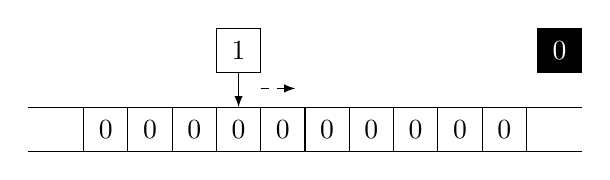
\begin{tikzpicture}[every node/.style={block},
				block/.style={minimum size=1.6em,outer sep=0pt,draw,rectangle,node distance=0pt}]
				\node (A)                         {0};
				\node (B)     [right=of A]        {0};
				\node (C)     [right=of B]        {0};
				\node (D)     [right=of C]        {0};
				\node (E)     [right=of D]        {0};
				\node (F)     [right=of E]        {0};
				\node (G)     [right=of F]        {0};
				\node (H)     [right=of G]        {0};
				\node (I)     [right=of H]        {0};
				\node (Z)     [right=of I]        {0};
				\node (HEAD)  [above=1.25em of D] {1};
				\node (STATE) [fill=black] at ([shift={(54.9406:3.4817em)}]Z) {\color{white}0};
				
				\draw[-latex]        (HEAD) -- (D);
				\draw[-latex,dashed] ([yshift=-1.375em]HEAD.east) -- ++(1.25em,0);
				\draw (A.north west) -- ++(-2em,0) (A.south west) -- ++ (-2em,0)
					(Z.north east) -- ++(2em,0) (Z.south east) -- ++ (2em,0);
			\end{tikzpicture}
		\end{center}
		\begin{center}
			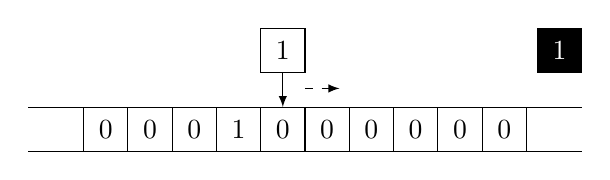
\begin{tikzpicture}[every node/.style={block},
				block/.style={minimum size=1.6em,outer sep=0pt,draw,rectangle,node distance=0pt}]
				\node (A)                         {0};
				\node (B)     [right=of A]        {0};
				\node (C)     [right=of B]        {0};
				\node (D)     [right=of C]        {1};
				\node (E)     [right=of D]        {0};
				\node (F)     [right=of E]        {0};
				\node (G)     [right=of F]        {0};
				\node (H)     [right=of G]        {0};
				\node (I)     [right=of H]        {0};
				\node (Z)     [right=of I]        {0};
				\node (HEAD)  [above=1.25em of E] {1};
				\node (STATE) [fill=black] at ([shift={(54.9406:3.4817em)}]Z) {\color{white}1};
				
				\draw[-latex]        (HEAD) -- (E);
				\draw[-latex,dashed] ([yshift=-1.375em]HEAD.east) -- ++(1.25em,0);
				\draw (A.north west) -- ++(-2em,0) (A.south west) -- ++ (-2em,0)
					(Z.north east) -- ++(2em,0) (Z.south east) -- ++ (2em,0);
			\end{tikzpicture}
			
			\phantom{This is meant to be a new line lol}
			
			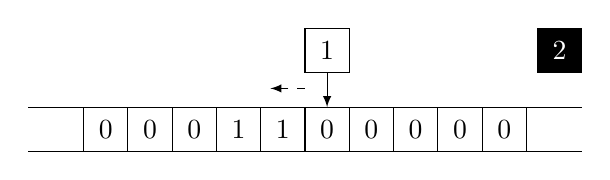
\begin{tikzpicture}[every node/.style={block},
				block/.style={minimum size=1.6em,outer sep=0pt,draw,rectangle,node distance=0pt}]
				\node (A)                         {0};
				\node (B)     [right=of A]        {0};
				\node (C)     [right=of B]        {0};
				\node (D)     [right=of C]        {1};
				\node (E)     [right=of D]        {1};
				\node (F)     [right=of E]        {0};
				\node (G)     [right=of F]        {0};
				\node (H)     [right=of G]        {0};
				\node (I)     [right=of H]        {0};
				\node (Z)     [right=of I]        {0};
				\node (HEAD)  [above=1.25em of F] {1};
				\node (STATE) [fill=black] at ([shift={(54.9406:3.4817em)}]Z) {\color{white}2};
				
				\draw[-latex]        (HEAD) -- (F);
				\draw[-latex,dashed] ([yshift=-1.375em]HEAD.west) -- ++(-1.25em,0);
				\draw (A.north west) -- ++(-2em,0) (A.south west) -- ++ (-2em,0)
					(Z.north east) -- ++(2em,0) (Z.south east) -- ++ (2em,0);
			\end{tikzpicture}
			
			\phantom{This is meant to be a new line lol}
			
			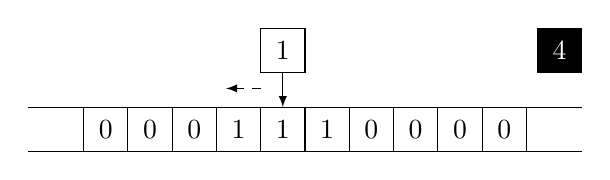
\begin{tikzpicture}[every node/.style={block},
				block/.style={minimum size=1.6em,outer sep=0pt,draw,rectangle,node distance=0pt}]
				\node (A)                         {0};
				\node (B)     [right=of A]        {0};
				\node (C)     [right=of B]        {0};
				\node (D)     [right=of C]        {1};
				\node (E)     [right=of D]        {1};
				\node (F)     [right=of E]        {1};
				\node (G)     [right=of F]        {0};
				\node (H)     [right=of G]        {0};
				\node (I)     [right=of H]        {0};
				\node (Z)     [right=of I]        {0};
				\node (HEAD)  [above=1.25em of E] {1};
				\node (STATE) [fill=black] at ([shift={(54.9406:3.4817em)}]Z) {\color{white}4};
				
				\draw[-latex]        (HEAD) -- (E);
				\draw[-latex,dashed] ([yshift=-1.375em]HEAD.west) -- ++(-1.25em,0);
				\draw (A.north west) -- ++(-2em,0) (A.south west) -- ++ (-2em,0)
					(Z.north east) -- ++(2em,0) (Z.south east) -- ++ (2em,0);
			\end{tikzpicture}
		\end{center}
		
		Now suppose the tape reads $0(1110)^n1110$ after $10n + 3$ steps. Then, by the induction hypothesis, the Turing machine will be as shown below.
		\begin{center}
			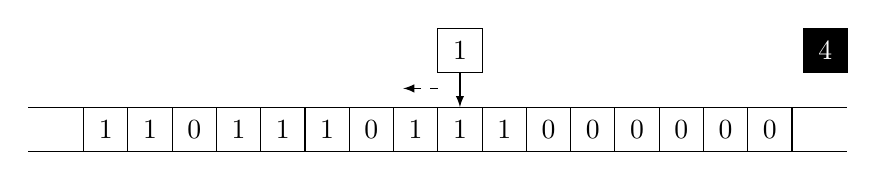
\begin{tikzpicture}[every node/.style={block},
				block/.style={minimum size=1.6em,outer sep=0pt,draw,rectangle,node distance=0pt}]
				\node (A)                         {1};
				\node (B)     [right=of A]        {1};
				\node (C)     [right=of B]        {0};
				\node (D)     [right=of C]        {1};
				\node (E)     [right=of D]        {1};
				\node (F)     [right=of E]        {1};
				\node (G)     [right=of F]        {0};
				\node (H)     [right=of G]        {1};
				\node (I)     [right=of H]        {1};
				\node (J)     [right=of I]        {1};
				\node (K)     [right=of J]        {0};
				\node (L)     [right=of K]        {0};
				\node (M)     [right=of L]        {0};
				\node (N)     [right=of M]        {0};
				\node (O)     [right=of N]        {0};
				\node (Z)     [right=of O]        {0};
				\node (HEAD)  [above=1.25em of I] {1};
				\node (STATE) [fill=black] at ([shift={(54.9406:3.4817em)}]Z) {\color{white}4};
				
				\draw[-latex]        (HEAD) -- (I);
				\draw[-latex,dashed] ([yshift=-1.375em]HEAD.west) -- ++(-1.25em,0);
				\draw (A.north west) -- ++(-2em,0) (A.south west) -- ++ (-2em,0)
					(Z.north east) -- ++(2em,0) (Z.south east) -- ++ (2em,0);
			\end{tikzpicture}
		\end{center}
		Tracing through the next 10 steps, to make $10(n+1) + 3$ steps in total, we have the following.
		\begin{center}
			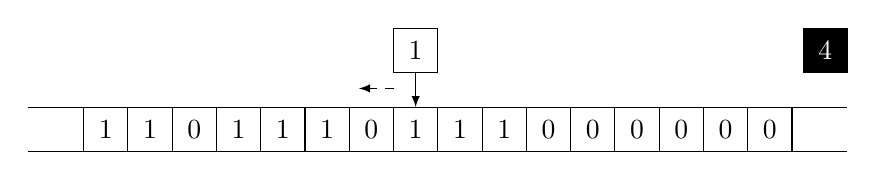
\begin{tikzpicture}[every node/.style={block},
				block/.style={minimum size=1.6em,outer sep=0pt,draw,rectangle,node distance=0pt}]
				\node (A)                         {1};
				\node (B)     [right=of A]        {1};
				\node (C)     [right=of B]        {0};
				\node (D)     [right=of C]        {1};
				\node (E)     [right=of D]        {1};
				\node (F)     [right=of E]        {1};
				\node (G)     [right=of F]        {0};
				\node (H)     [right=of G]        {1};
				\node (I)     [right=of H]        {1};
				\node (J)     [right=of I]        {1};
				\node (K)     [right=of J]        {0};
				\node (L)     [right=of K]        {0};
				\node (M)     [right=of L]        {0};
				\node (N)     [right=of M]        {0};
				\node (O)     [right=of N]        {0};
				\node (Z)     [right=of O]        {0};
				\node (HEAD)  [above=1.25em of H] {1};
				\node (STATE) [fill=black] at ([shift={(54.9406:3.4817em)}]Z) {\color{white}4};
				
				\draw[-latex]        (HEAD) -- (H);
				\draw[-latex,dashed] ([yshift=-1.375em]HEAD.west) -- ++(-1.25em,0);
				\draw (A.north west) -- ++(-2em,0) (A.south west) -- ++ (-2em,0)
					(Z.north east) -- ++(2em,0) (Z.south east) -- ++ (2em,0);
			\end{tikzpicture}
			
			\phantom{This is meant to be a new line lol}
			
			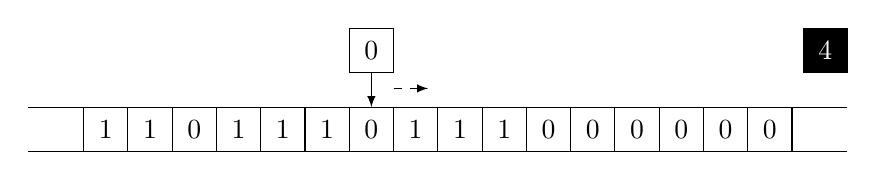
\begin{tikzpicture}[every node/.style={block},
				block/.style={minimum size=1.6em,outer sep=0pt,draw,rectangle,node distance=0pt}]
				\node (A)                         {1};
				\node (B)     [right=of A]        {1};
				\node (C)     [right=of B]        {0};
				\node (D)     [right=of C]        {1};
				\node (E)     [right=of D]        {1};
				\node (F)     [right=of E]        {1};
				\node (G)     [right=of F]        {0};
				\node (H)     [right=of G]        {1};
				\node (I)     [right=of H]        {1};
				\node (J)     [right=of I]        {1};
				\node (K)     [right=of J]        {0};
				\node (L)     [right=of K]        {0};
				\node (M)     [right=of L]        {0};
				\node (N)     [right=of M]        {0};
				\node (O)     [right=of N]        {0};
				\node (Z)     [right=of O]        {0};
				\node (HEAD)  [above=1.25em of G] {0};
				\node (STATE) [fill=black] at ([shift={(54.9406:3.4817em)}]Z) {\color{white}4};
				
				\draw[-latex]        (HEAD) -- (G);
				\draw[-latex,dashed] ([yshift=-1.375em]HEAD.east) -- ++(1.25em,0);
				\draw (A.north west) -- ++(-2em,0) (A.south west) -- ++ (-2em,0)
					(Z.north east) -- ++(2em,0) (Z.south east) -- ++ (2em,0);
			\end{tikzpicture}
			
			\phantom{This is meant to be a new line lol}
			
			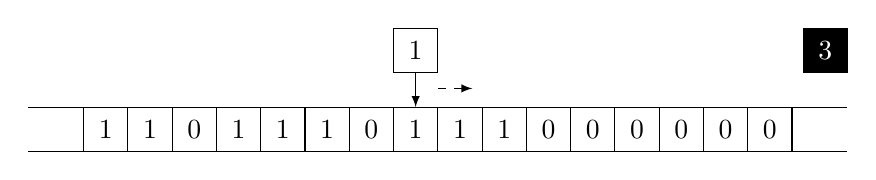
\begin{tikzpicture}[every node/.style={block},
				block/.style={minimum size=1.6em,outer sep=0pt,draw,rectangle,node distance=0pt}]
				\node (A)                         {1};
				\node (B)     [right=of A]        {1};
				\node (C)     [right=of B]        {0};
				\node (D)     [right=of C]        {1};
				\node (E)     [right=of D]        {1};
				\node (F)     [right=of E]        {1};
				\node (G)     [right=of F]        {0};
				\node (H)     [right=of G]        {1};
				\node (I)     [right=of H]        {1};
				\node (J)     [right=of I]        {1};
				\node (K)     [right=of J]        {0};
				\node (L)     [right=of K]        {0};
				\node (M)     [right=of L]        {0};
				\node (N)     [right=of M]        {0};
				\node (O)     [right=of N]        {0};
				\node (Z)     [right=of O]        {0};
				\node (HEAD)  [above=1.25em of H] {1};
				\node (STATE) [fill=black] at ([shift={(54.9406:3.4817em)}]Z) {\color{white}3};
				
				\draw[-latex]        (HEAD) -- (H);
				\draw[-latex,dashed] ([yshift=-1.375em]HEAD.east) -- ++(1.25em,0);
				\draw (A.north west) -- ++(-2em,0) (A.south west) -- ++ (-2em,0)
					(Z.north east) -- ++(2em,0) (Z.south east) -- ++ (2em,0);
			\end{tikzpicture}
			
			\phantom{This is meant to be a new line lol}
			
			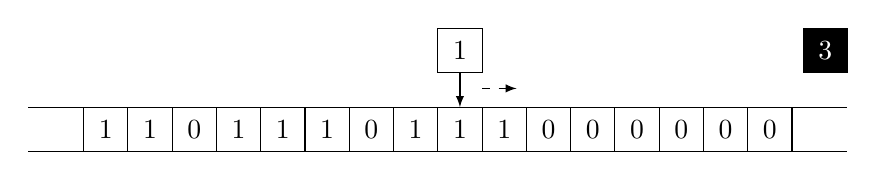
\begin{tikzpicture}[every node/.style={block},
				block/.style={minimum size=1.6em,outer sep=0pt,draw,rectangle,node distance=0pt}]
				\node (A)                         {1};
				\node (B)     [right=of A]        {1};
				\node (C)     [right=of B]        {0};
				\node (D)     [right=of C]        {1};
				\node (E)     [right=of D]        {1};
				\node (F)     [right=of E]        {1};
				\node (G)     [right=of F]        {0};
				\node (H)     [right=of G]        {1};
				\node (I)     [right=of H]        {1};
				\node (J)     [right=of I]        {1};
				\node (K)     [right=of J]        {0};
				\node (L)     [right=of K]        {0};
				\node (M)     [right=of L]        {0};
				\node (N)     [right=of M]        {0};
				\node (O)     [right=of N]        {0};
				\node (Z)     [right=of O]        {0};
				\node (HEAD)  [above=1.25em of I] {1};
				\node (STATE) [fill=black] at ([shift={(54.9406:3.4817em)}]Z) {\color{white}3};
				
				\draw[-latex]        (HEAD) -- (I);
				\draw[-latex,dashed] ([yshift=-1.375em]HEAD.east) -- ++(1.25em,0);
				\draw (A.north west) -- ++(-2em,0) (A.south west) -- ++ (-2em,0)
					(Z.north east) -- ++(2em,0) (Z.south east) -- ++ (2em,0);
			\end{tikzpicture}
			
			\phantom{This is meant to be a new line lol}
			
			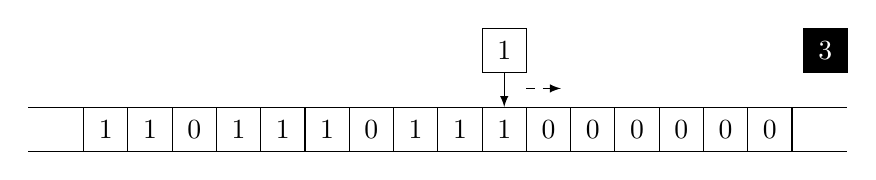
\begin{tikzpicture}[every node/.style={block},
				block/.style={minimum size=1.6em,outer sep=0pt,draw,rectangle,node distance=0pt}]
				\node (A)                         {1};
				\node (B)     [right=of A]        {1};
				\node (C)     [right=of B]        {0};
				\node (D)     [right=of C]        {1};
				\node (E)     [right=of D]        {1};
				\node (F)     [right=of E]        {1};
				\node (G)     [right=of F]        {0};
				\node (H)     [right=of G]        {1};
				\node (I)     [right=of H]        {1};
				\node (J)     [right=of I]        {1};
				\node (K)     [right=of J]        {0};
				\node (L)     [right=of K]        {0};
				\node (M)     [right=of L]        {0};
				\node (N)     [right=of M]        {0};
				\node (O)     [right=of N]        {0};
				\node (Z)     [right=of O]        {0};
				\node (HEAD)  [above=1.25em of J] {1};
				\node (STATE) [fill=black] at ([shift={(54.9406:3.4817em)}]Z) {\color{white}3};
				
				\draw[-latex]        (HEAD) -- (J);
				\draw[-latex,dashed] ([yshift=-1.375em]HEAD.east) -- ++(1.25em,0);
				\draw (A.north west) -- ++(-2em,0) (A.south west) -- ++ (-2em,0)
					(Z.north east) -- ++(2em,0) (Z.south east) -- ++ (2em,0);
			\end{tikzpicture}
			
			\phantom{This is meant to be a new line lol}
			
			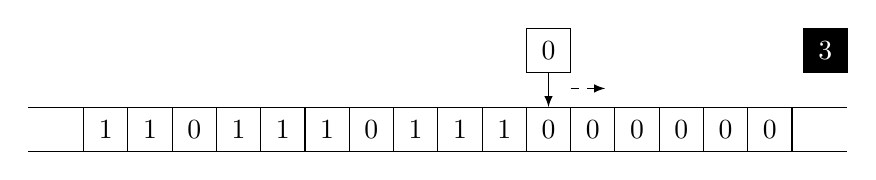
\begin{tikzpicture}[every node/.style={block},
				block/.style={minimum size=1.6em,outer sep=0pt,draw,rectangle,node distance=0pt}]
				\node (A)                         {1};
				\node (B)     [right=of A]        {1};
				\node (C)     [right=of B]        {0};
				\node (D)     [right=of C]        {1};
				\node (E)     [right=of D]        {1};
				\node (F)     [right=of E]        {1};
				\node (G)     [right=of F]        {0};
				\node (H)     [right=of G]        {1};
				\node (I)     [right=of H]        {1};
				\node (J)     [right=of I]        {1};
				\node (K)     [right=of J]        {0};
				\node (L)     [right=of K]        {0};
				\node (M)     [right=of L]        {0};
				\node (N)     [right=of M]        {0};
				\node (O)     [right=of N]        {0};
				\node (Z)     [right=of O]        {0};
				\node (HEAD)  [above=1.25em of K] {0};
				\node (STATE) [fill=black] at ([shift={(54.9406:3.4817em)}]Z) {\color{white}3};
				
				\draw[-latex]        (HEAD) -- (K);
				\draw[-latex,dashed] ([yshift=-1.375em]HEAD.east) -- ++(1.25em,0);
				\draw (A.north west) -- ++(-2em,0) (A.south west) -- ++ (-2em,0)
					(Z.north east) -- ++(2em,0) (Z.south east) -- ++ (2em,0);
			\end{tikzpicture}
			
			\phantom{This is meant to be a new line lol}
			
			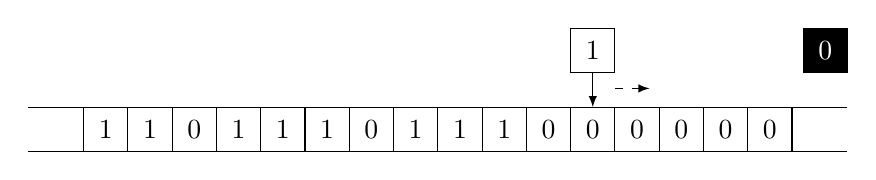
\begin{tikzpicture}[every node/.style={block},
				block/.style={minimum size=1.6em,outer sep=0pt,draw,rectangle,node distance=0pt}]
				\node (A)                         {1};
				\node (B)     [right=of A]        {1};
				\node (C)     [right=of B]        {0};
				\node (D)     [right=of C]        {1};
				\node (E)     [right=of D]        {1};
				\node (F)     [right=of E]        {1};
				\node (G)     [right=of F]        {0};
				\node (H)     [right=of G]        {1};
				\node (I)     [right=of H]        {1};
				\node (J)     [right=of I]        {1};
				\node (K)     [right=of J]        {0};
				\node (L)     [right=of K]        {0};
				\node (M)     [right=of L]        {0};
				\node (N)     [right=of M]        {0};
				\node (O)     [right=of N]        {0};
				\node (Z)     [right=of O]        {0};
				\node (HEAD)  [above=1.25em of L] {1};
				\node (STATE) [fill=black] at ([shift={(54.9406:3.4817em)}]Z) {\color{white}0};
				
				\draw[-latex]        (HEAD) -- (L);
				\draw[-latex,dashed] ([yshift=-1.375em]HEAD.east) -- ++(1.25em,0);
				\draw (A.north west) -- ++(-2em,0) (A.south west) -- ++ (-2em,0)
					(Z.north east) -- ++(2em,0) (Z.south east) -- ++ (2em,0);
			\end{tikzpicture}
			
			\phantom{This is meant to be a new line lol}
			
			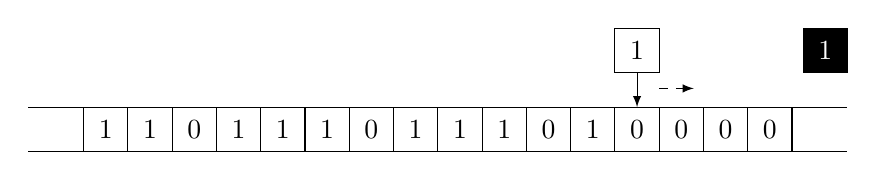
\begin{tikzpicture}[every node/.style={block},
				block/.style={minimum size=1.6em,outer sep=0pt,draw,rectangle,node distance=0pt}]
				\node (A)                         {1};
				\node (B)     [right=of A]        {1};
				\node (C)     [right=of B]        {0};
				\node (D)     [right=of C]        {1};
				\node (E)     [right=of D]        {1};
				\node (F)     [right=of E]        {1};
				\node (G)     [right=of F]        {0};
				\node (H)     [right=of G]        {1};
				\node (I)     [right=of H]        {1};
				\node (J)     [right=of I]        {1};
				\node (K)     [right=of J]        {0};
				\node (L)     [right=of K]        {1};
				\node (M)     [right=of L]        {0};
				\node (N)     [right=of M]        {0};
				\node (O)     [right=of N]        {0};
				\node (Z)     [right=of O]        {0};
				\node (HEAD)  [above=1.25em of M] {1};
				\node (STATE) [fill=black] at ([shift={(54.9406:3.4817em)}]Z) {\color{white}1};
				
				\draw[-latex]        (HEAD) -- (M);
				\draw[-latex,dashed] ([yshift=-1.375em]HEAD.east) -- ++(1.25em,0);
				\draw (A.north west) -- ++(-2em,0) (A.south west) -- ++ (-2em,0)
					(Z.north east) -- ++(2em,0) (Z.south east) -- ++ (2em,0);
			\end{tikzpicture}
			
			\phantom{This is meant to be a new line lol}
			
			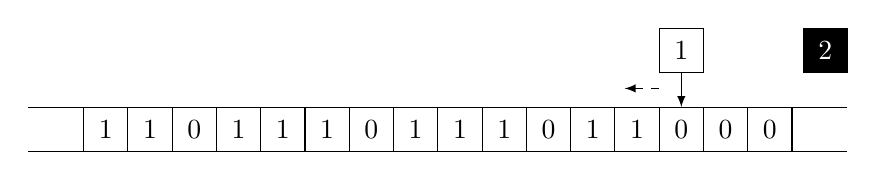
\begin{tikzpicture}[every node/.style={block},
				block/.style={minimum size=1.6em,outer sep=0pt,draw,rectangle,node distance=0pt}]
				\node (A)                         {1};
				\node (B)     [right=of A]        {1};
				\node (C)     [right=of B]        {0};
				\node (D)     [right=of C]        {1};
				\node (E)     [right=of D]        {1};
				\node (F)     [right=of E]        {1};
				\node (G)     [right=of F]        {0};
				\node (H)     [right=of G]        {1};
				\node (I)     [right=of H]        {1};
				\node (J)     [right=of I]        {1};
				\node (K)     [right=of J]        {0};
				\node (L)     [right=of K]        {1};
				\node (M)     [right=of L]        {1};
				\node (N)     [right=of M]        {0};
				\node (O)     [right=of N]        {0};
				\node (Z)     [right=of O]        {0};
				\node (HEAD)  [above=1.25em of N] {1};
				\node (STATE) [fill=black] at ([shift={(54.9406:3.4817em)}]Z) {\color{white}2};
				
				\draw[-latex]        (HEAD) -- (N);
				\draw[-latex,dashed] ([yshift=-1.375em]HEAD.west) -- ++(-1.25em,0);
				\draw (A.north west) -- ++(-2em,0) (A.south west) -- ++ (-2em,0)
					(Z.north east) -- ++(2em,0) (Z.south east) -- ++ (2em,0);
			\end{tikzpicture}
			
			\phantom{This is meant to be a new line lol}
			
			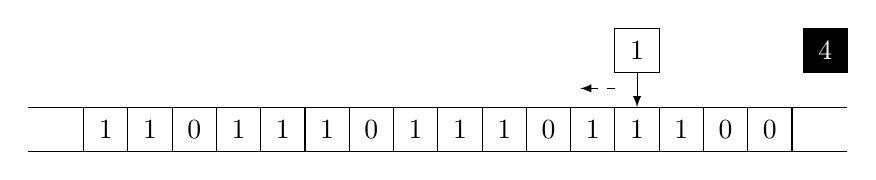
\begin{tikzpicture}[every node/.style={block},
				block/.style={minimum size=1.6em,outer sep=0pt,draw,rectangle,node distance=0pt}]
				\node (A)                         {1};
				\node (B)     [right=of A]        {1};
				\node (C)     [right=of B]        {0};
				\node (D)     [right=of C]        {1};
				\node (E)     [right=of D]        {1};
				\node (F)     [right=of E]        {1};
				\node (G)     [right=of F]        {0};
				\node (H)     [right=of G]        {1};
				\node (I)     [right=of H]        {1};
				\node (J)     [right=of I]        {1};
				\node (K)     [right=of J]        {0};
				\node (L)     [right=of K]        {1};
				\node (M)     [right=of L]        {1};
				\node (N)     [right=of M]        {1};
				\node (O)     [right=of N]        {0};
				\node (Z)     [right=of O]        {0};
				\node (HEAD)  [above=1.25em of M] {1};
				\node (STATE) [fill=black] at ([shift={(54.9406:3.4817em)}]Z) {\color{white}4};
				
				\draw[-latex]        (HEAD) -- (M);
				\draw[-latex,dashed] ([yshift=-1.375em]HEAD.west) -- ++(-1.25em,0);
				\draw (A.north west) -- ++(-2em,0) (A.south west) -- ++ (-2em,0)
					(Z.north east) -- ++(2em,0) (Z.south east) -- ++ (2em,0);
			\end{tikzpicture}
		\end{center}
		Thus, after $10n + 3$ steps the machine will be in state [4] with the tape reading $\ldots 0(1110)^n1\underset{\uparrow}{1}10 \ldots$
	\end{enumerate}
\end{document}
